\chapter{Theory}
\label{chap:theory}

\section{2D Image Processing}

Image processing describes the application of different algorithms on images with the purpose of gaining certain information about it or changing its representation. Most of the time images are given as two dimensional pixel arrays where each entry denotes the intensity of that pixel. In the case of grayscale images the value is between 0 and 255 representing black and white respectively. When handling color images an additional 3rd dimension is added with three channels representing a red, green, blue (rgb) encoding. Each entry, again, has values between 0 and 255 representing color intensity. \\
Instead of imagining an image as a flat 2D object, it can also be seen as a terrain with surface, where the height of each coordinate is determined by the intensity of its value. An example of this is shown in figure \ref{fig:image_surfaces}. 


\begin{figure}[!htb]
	\centering
	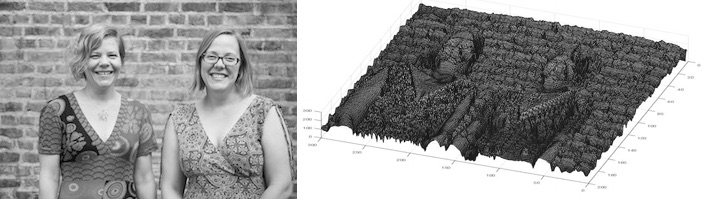
\includegraphics[width = 0.9\textwidth]{images/image_surfaces.jpg}
	\caption{Left: image represented as 2D flat surface. Right: image as 3D terrain with uneven surface. \protect\footnotemark}
	\label{fig:image_surfaces}
\end{figure}

\footnotetext{Figure taken from \url{https://plus.maths.org/content/fourier-transforms-images}}

%how does this work for color images?
%-> see scaling the scattering transform, just use 3 channels

Like every other surface, these images can now be approximated as the sum of many different two dimensional sine waves. 2D sine waves are defined as in equation \ref{eq:2d_sine}, where f $a$ is the amplitude and $h, k$ are the frequencies in $x$ and $y$ direction respectively.

\begin{equation}
	f = a \sin(h\cdot x+k\cdot y)
	\label{eq:2d_sine}
\end{equation}

To give an example of how this approximation looks like, figure \ref{fig:2d_sine} shows examples of three different two dimensional sine waves. It can be observes that higher amplitudes dominate the resulting wave, i.e. determine the direction of the wave stronger than the smaller amplitudes. 


\begin{figure}[!htb]
	\centering
	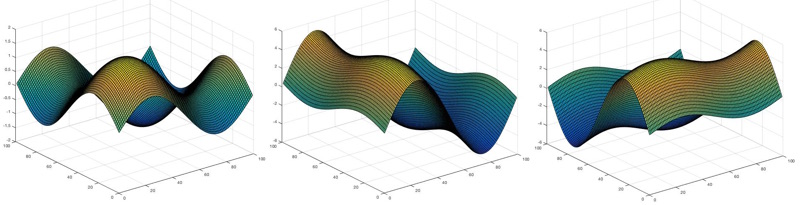
\includegraphics[width = \textwidth]{images/2d_sine.jpg}
	\caption{Left: $\sin(x) +\sin(y)$. Middle:  $5 \sin(x)+ \sin(y)$. Right: $	\sin(x)+5\sin(y)$. On the middle and right images the higher amplitudes of 5 dominate the resulting wave. \protect\footnotemark}
	\label{fig:2d_sine}
\end{figure}

\footnotetext{Figure taken from \url{https://plus.maths.org/content/fourier-transforms-images}}

\section{Fourier Transformation}

A Fourier Transform (FT) decomposes a signal into the frequencies that make it up.
\subsection{One dimensional FT} 

In the case of one dimensional signals the decomposition are the coefficients of the sine waves representing the signal. A good example of this would be the decomposition of a  The FT is defined by equation \ref{eq:forward_FT} for any real number $\omega$ and any integrable function $f:\mathbb{R} \rightarrow \mathbb{C}$. 

\begin{equation}
	\tilde{f}(\omega) = \int_{-\infty}^{\infty} f(x)\ e^{-2\pi i x \omega}dx
	\label{eq:forward_FT}
\end{equation} 

To get back to the Fourier domain when the given a frequency, the inverse Fourier transform defined in equation \ref{eq:inverse_FT} is used.  \\

\begin{equation}
	f(x) = \int_{-\infty}^{\infty} \tilde{f}(\omega)\ e^{2 \pi i x \omega}d\omega
	\label{eq:inverse_FT}
\end{equation}

When using discrete instead of continuous functions, the integrals in the definitions become sums. Then the definition of the forward FT is given in equation \ref{eq:forward_FT_dis} and in equation \ref{eq:inverse_FT_dis} for the inverse FT. 

\begin{equation}
\tilde{f}(\omega) = \sum_{x=1}^{n} f(x)\ e^{-2\pi i x \omega}
\label{eq:forward_FT_dis}
\end{equation} 

\begin{equation}
f(x) = \sum_{x=1}^{n} \tilde{f}(\omega)\ e^{2 \pi i x \omega}
\label{eq:inverse_FT_dis}
\end{equation}

\subsection{Two dimensional FT}

Since images are two dimensional objects the Fourier transform needs to be extended. The Fourier transform then becomes a complex function of two or more real frequency variables $\omega_1, \omega_2$. Since images images are finite objects the discrete version of the two dimensional Fourier transform is given in equation \ref{eq:forward_FT_2D} for the forward case and in equation \ref{eq:inverse_FT_2D} for the inverse case.

\begin{equation}
	\tilde{f}(\omega_1, \omega_2) = \sum_{x=1}^{n} \sum_{y=1}^{m} f(x,y)\ e^{-2\pi i (\omega_1 \cdot x + \omega_2 \cdot y)}
\label{eq:forward_FT_2D}
\end{equation}

\begin{equation}
f(x, y) = \sum_{x=1}^{n} \sum_{y=1}^{m} \tilde{f}(\omega_1, \omega_2)\ e^{2\pi i (\omega_1 \cdot x + \omega_2 \cdot y)}
\label{eq:inverse_FT_2D}
\end{equation}

\section{Object detection}

Object detection is a task within image processing where objects on a given image are supposed to be detected. These objects can be anything from buildings over cars to humans. The images are already annotated for training, i.e. a rectangle (or other representation) that approximates the object best is already placed over the picture with the associated class attached. An example of such an annotated image can be found in figure \ref*{fig:annot_example}.

\begin{figure}[!htb]
	\centering
	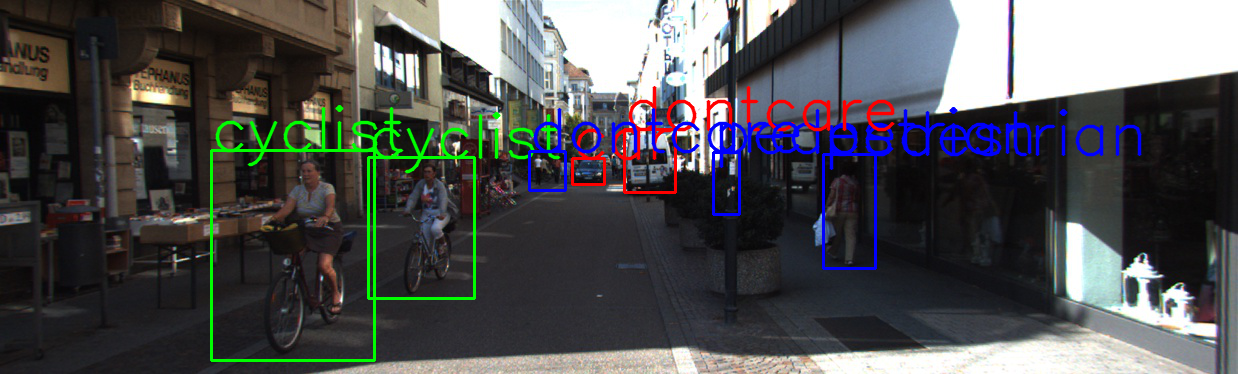
\includegraphics[width=0.9\textwidth]{images/Annotations_example.png}
	\caption{An example of a annotated image taken from the Kitti dataset. There are seven objects of four classes visible: cyclist, car, pedestrian and dontcare.}
	\label{fig:annot_example}
\end{figure}

Many methods have been explored to increase the accuracy of object detection ranging from sliding window approaches (citation needed) over hand crafted feature extraction (citation needed) to artificial neural networks. All current state of the art results for object detection are achieved by using Convolutional Neural Networks (CNN) with minor or major adaptions (citation needed). Therefore this work also uses a CNN as the backbone of the object detection.
     
\section{Convolutional Neural Networks}

For most image-related tasks, i.e. classification or object detection, a picture is used as a collection of pixels. However, not all pixels are equally important and subsets of the entire image form meaningfully connected subcollections. This might be a face in a photo of a family gathering. For humans the ability to detect these features and contextualize them comes naturally, for computers it does not. Therefore convolutional neural networks (CNNs) \cite{LeCun1989BackpropagationAT} are used. Convolutions are essentially just the application of filters on an image. The filter is applied at every possible location in the image, as described in figure: 

\begin{figure}[!htb]
	\centering
	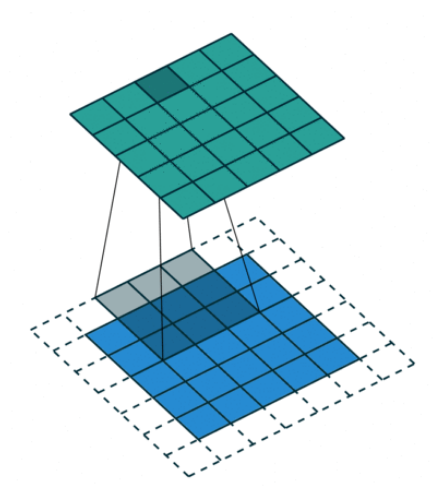
\includegraphics[width=0.5\textwidth]{images/convolution.png}
	\caption{3x3 convolution on 5x5 image. Resulting image is also 5x5 due to the padding of size 1 added on original image. \protect\footnotemark}
	\label{fig:convolution}
\end{figure}

\footnotetext{Figure taken from and animated version at \url{https://towardsdatascience.com/types-of-convolutions-in-deep-learning-717013397f4d}}

In CNNs there are multiple stages of filters in sequential order and multiple filters per layer. That means at every stage of the network different filters are applied on the outcome of an earlier step. The filters are assumed to learn different features of the images. The later the stage, the higher the level of complexity of the feature to be learned. That means, that an early filter might learn simple attributes such as edges or colors while a later filter might learn more complex features such as an eye or a nose and the very last filters even more complex semantic objects such as a face. The weights that are adapted during training determine what each individual filter does. This means that every filter that is a applied on a given layer learns its specific function such that overall the best accuracy can be achieved. 

As just explained in conventional CNNs the filters are trained. However, there are some approaches that use static filters. The Scattering Transform is one of those approaches. Given its unique properties the results might be comparable to the conventional approach. If weights are not trained a lot of time can be saved. 

\section{Scattering Transform}

A transformation from the Fourier to the frequency domain cannot only be performed by using the sine but in principal with any given periodic function.
Wavelets are wave-like oscillation with an amplitude that begin and end at zero. In most use cases wavelets are specifically crafted to have certain properties. 
The Scattering Transform is based on a Morlet wavelet, which is defined in equation \ref{eq:morlet2d}.

\begin{equation}
	\psi(u) = C_1 (e^{iu.\xi} - C_2) e^{\frac{-|u|^2}{2\sigma^2}}
	\label{eq:morlet2d}
\end{equation}

%TODO: what is the meaning of all those symbols?

where $C_2$ is chosen such that $\int \psi(u) du = 0$. $u.\xi$ denotes the innerproduct of $u$ and $\xi$ and $|u|^2$ is the norm in $\mathbb{R}^2$. 
%TODO: what is sigma
%TODO: what is xi
%TODO: what is C_1 and C_2
Figure \ref{fig:morlet2d} shows the 2 dimensional Morlet wavelet with parameters $\sigma = 0.85$ and $\xi = \frac{3\pi}{4}$. These parameters are taken from \cite{scatteringTransform2012}. No additional fine tuning w.r.t. to these parameters is done in this work. 

\begin{figure}[!htb]
	\centering
	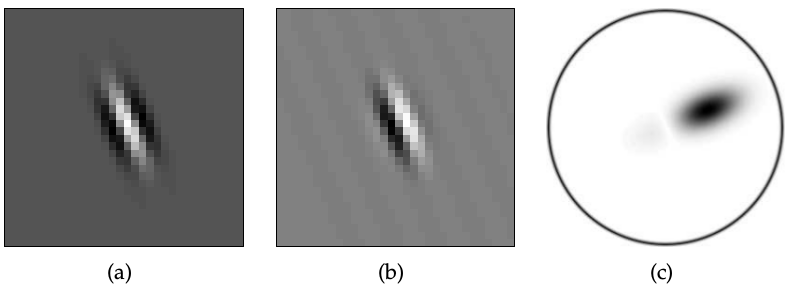
\includegraphics[width = 0.9\textwidth]{images/morlet2d.png}
	\caption{Complex morlet wavelet. a) Real part of $\psi$. b) Imaginary part of $\psi$. c) Fourier modulus $|\hat{\psi}|$. Image taken from \cite{scatteringTransform2012}.}
	\label{fig:morlet2d}
\end{figure}

\subsection{Filter Bank}

A wavelet transform filters $x$ using a family of wavelets: $\{x \star \psi_\lambda (u)\}_\lambda$. It is computed with a filter bank of dilated and rotated wavelets having no orthogonality property. The filter bank has 4 parameters: $M, N, J, L$ where $M,N$ stand for the initial spatial size of the input, $J$ is the scaling parameter and $L$ is the number of angles used for the wavelet transform. $J$ determines the size of the downsampling for the filters. The new output is downsampled by $2^{2*J}$, i.e. An input image of size $(32, 32)$ is downsampled by $J=1$ to be of size $(16,16)$ or by $J=2$ to be of size $(8,8)$. It is important to note that the filter bank is just an accumulation of filters and is independent of the data. \\
A visualization of the filter bank used in this work can be found in figure \ref{fig:viz_filter_bank}. The filters are shown for $J=0,1,2$ and $L=8$ different angles. The red blurry dot in the bottom is the result of a Gabor filter which is a sinosoidal wave multiplied with a Gaussian function. The Gabor Filter is used as a low-pass filter.


\begin{figure}[!htb]
	\centering
	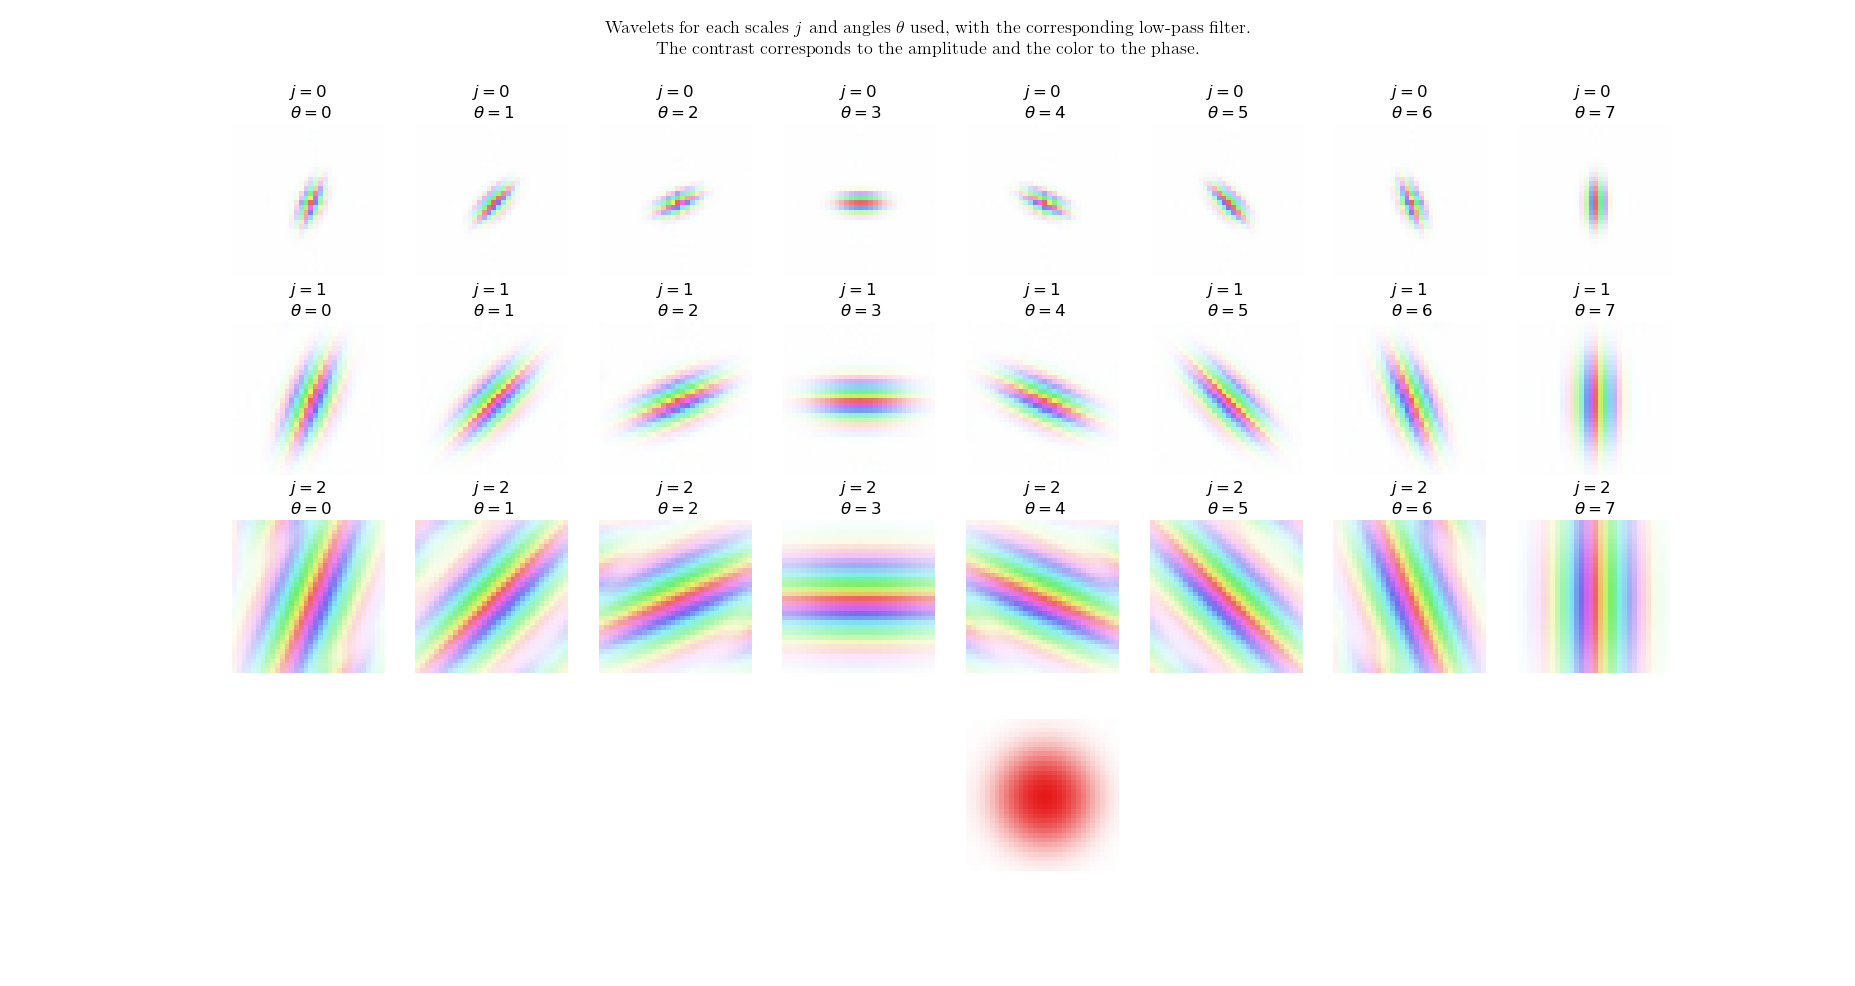
\includegraphics[width=\textwidth]{images/filter_bank_vis.png}
	\caption{Visualization of the filter bank. The $j=0,1,2$ describe the different downsample sizes. The $\theta=0,...,7$ describe the different angles. For these images $N,M=32, L=8, J=3$.}
    \label{fig:viz_filter_bank}
\end{figure}


\subsection{Scattering Paths}
\label{subsec:scattering_path}

To compute more and higher order scattering coefficients we iteratively apply the scattering transform. Let $U[\lambda]x = |x \star \psi_\lambda|$. A sequence $p = (\lambda_1, \lambda_2, ... \lambda_m)$ defines a \textit{path}, which is the ordered product: 
$$U[p]x = U[\lambda_m]...U[\lambda_2]U[\lambda_1] = | ||x \star \psi_{\lambda_1} | \star \psi_{\lambda_2}| ... | \star \psi_{\lambda_m}|. $$

A scattering transform along the path $p$ is defined as an integral, normalized by the response of a Dirac:

$$\bar{S}x(p) = \mu_p^{-1} \int U[p]x(u)du)$$

with $\mu_p \int U[p] \delta(u) du$. From this it follows that each scattering coefficient $\bar{S}x(p)$ is invariant to a translation of $x$. The scattering is Lipschitz continuous to deformations as opposed to the Fourier transform modulus

%TODO what does that mean and what property does the Fourier transform modulus have?

\subsection{Scattering Networks}

Scattering Networks are the result of all previously explained concepts. There are $m$ layers in the network, where every $m$ describes the length of the scattering paths in that layer. $m$ is also called order because it describes the number of consecutive scattering applications in that path. A scattering network is a tree that starts with a single root node in layer $m=0$ and branches out for every further layer with branching factor $L$. Similar to the filter bank the Scattering network is a collection of filters. However, the scattering network is the first time when data is actually input into those filters. In distinction to conventional CNNs the final output is not only taken from the last layer, but from every single node in that network. An example of a scattering network with $L=4$ and $m=3$ is shown in figure \ref{fig:scattering_network}. The nodes describe the filters that are independent of the data, i.e. $U[\lambda_1]f$ for the first layer. The black arrows indicate the outputs at every node, i.e. the scattering coefficients that result from applying this particular scattering path to data for example $S_J[\lambda_1]f$ for a node in the first layer. The root node $U_J[\theta]f = f \star \phi_J$ is the low-pass filter which is in this case a Gabor filter. \\
In \cite{scatteringTransform2012} it is shown that using more than $m=2$ produces a lot of unnecessary computation because most of the information from data is already captured in the second-order scattering coefficients. For practical purposes this paper from now on assumes that networks are at maximum $m=2$ layers deep and in this paper for some applications $m=1$ only. 
The total number of filters and therefore also the total number of outputs per datapoint are shown in 
\begin{equation}
	i \cdot (1 + JL) 
	\label{eq:order1_num_filters}
\end{equation} 
\begin{equation}
	i \cdot (1 + JL + \frac{1}{2}J(J-1)L^2)
	\label{eq:order2_num_filters}
\end{equation}
\ref{eq:order1_num_filters} for $m=1$ and in \ref{eq:order2_num_filters} for $m=2$. $i$ denotes the number of input channels of the input which is 3 for most applications since RGB images are used. In the case of RGB images the scattering transformation is applied for every channel separately. Figure \ref{fig:scattering_network} is only showing a network for one abstract $J$. In a real network this $J$ is an actual integer. Therefore it also has to be factored in the equations \ref{eq:order1_num_filters} and \ref{eq:order2_num_filters}. Lastly, it should be noted that the output of the scattering network all have the same downsamples size determined by $J$ even if the filters have different sizes. This is achieved by subsampling the current scattering coefficients in the Fourier domain such that the output is the desired one. To make this more clear an example is provided: A scattering network with $N,M = 32; J=2; L=8$ is initialized. The network is applied on an RGB image. Therefore there are $3*(1+2*8) = 51$ outputs of size $(8,8)$ because of the downsampling factor $J=2$. 
\begin{figure}[!htb]
	\centering
	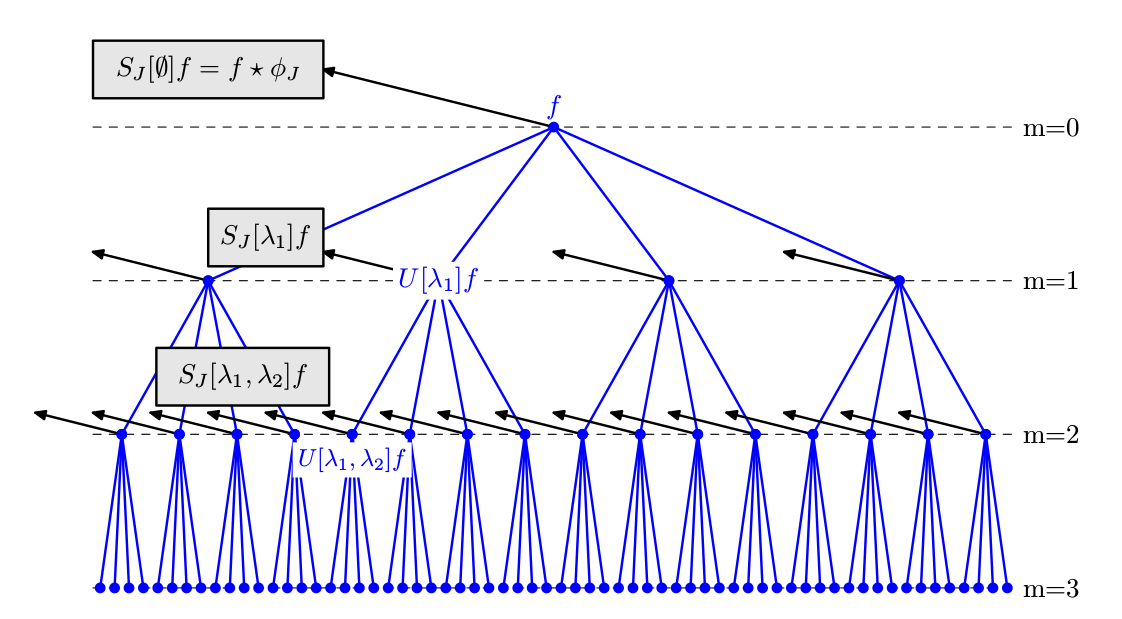
\includegraphics[width = 0.75\textwidth]{images/scattering_network.png}
	\caption{Representation of a scattering network. Each black arrow is an output of scattering coefficients of the specified path. The $m=0,1,2,3$ indicates the layer in the network, i.e. the number of iterations of the scattering transform.}
	\label{fig:scattering_network}
\end{figure}


\subsection{Properties of the Scattering Transform}

%TODO: How detailed? Just hint at it or copy entire section of original paper?
%-> rather detailed. everything should be clear

In this subsection the properties of the scattering transform as used in this work are layed out and the reasons for the properties are pointed out but not proven. For a more detailed explanation and references to proofs the original paper \cite{scatteringTransform2012} must be conducted. \\
A wavelet is a localized waveform and therefore stable to deformations. This is an upgrade to the sinusoidal waves of the Fourier transform which do not have this property. 
A wavelet transform computes convolutions with wavelets. It is thus translation covariant not invariant. To achieve invariance a non-linearity must be added. One can then show that the only non-linearity that fulfills the $\textbf{L}^2(\mathbb{R}^2)$ stability, is differentiable and commutes with translations is the $\textbf{L}^1(\mathbb{R}^2)$ norm. Therefore it is chosen as the non-linearity. \\
As already stated in its respective subsection \ref{subsec:scattering_path} a scattering transform along any scattering path is translation invariant. 
Compared to the Fourier transform modulus, which is also invariant to deformations, the scattering transform is Lipschitz continuous to deformations, i.e. the change in the scattering coefficients is bounded and determined by the change in the deformed object. \\
There are no theoretical bounds on the behavior of the scattering transform when confronted with scaled or rotated objects. However, there are some predictions one can make that will be layed out in the following. Given that scattering networks use rotated and dilated filters with $L$ different angles with equidistant spacing it seems plausible that rotated objects should be captured in some of the filters. Scaled objects should also be captured by the scattering network, because scaling can be viewed as a specific subset of deformation. The Lipschitz continuity w.r.t deformation should also benefit the detection of scaled objects. 

\subsubsection{Discussion of the properties}

In this work the scattering transform should be applied to object detection. In previous works the scattering transform has mainly been applied to image classification. In the following a short distinction between the two tasks is presented. For image classification invariance/Lipschitz continuity w.r.t. rotation, translation, scale and deformation are all positive attributes because every image corresponds to exactly one category. In the context of object detection invariance/Lipschitz continuity w.r.t. rotation, scale and deformation are positive attributes. However, the invariance w.r.t. translation is potentially very problematic. When two objects at two different locations in the image lead to exactly the same scattering coefficients it is impossible to detect these objects correctly. \\
Given this theoretical insight this work proposes a specific kind of hybrid network which includes information from both a conventional CNN and the scattering networks. 

\section{Hybrid Networks}

%TODO

\subsection{Sequential Hybrid Networks}

\subsection{Parallel Hybrid Networks}
